\documentclass[11pt,a4paper]{article}

\usepackage[utf8]{inputenc} 
\usepackage[T1]{fontenc} 
\usepackage{lmodern}
\usepackage[margin=2cm]{geometry}
\usepackage[german]{babel}
\usepackage{amsmath} 
\usepackage{graphicx} 
\usepackage{booktabs}
\usepackage{hyperref}
\hypersetup{
    colorlinks,
    citecolor=red,
    filecolor=black,
    linkcolor=black!20!blue!90!,
    urlcolor=black} 
\usepackage{nicefrac}
\usepackage[table]{xcolor}
\usepackage{tocloft}

\setlength{\parindent}{0pt}
\setlength{\parskip}{1ex plus 0.5ex minus 0.5ex}

\definecolor{incolor}{rgb}{0.0, 0.0, 0.5}

\hbadness=99999

\newcommand{\refpy}[1]{Siehe Anhang: \textit{Rechnungen in Python} (\texttt{{\color{incolor}In [{\color{incolor}#1}]}})}
\newcommand\dif{\mathop{}\!\mathrm{d}}
\newcommand{\halftime}[4]{\begin{figure}[h]
\begin{minipage}{.#1\textwidth}#3\end{minipage}\begin{minipage}{.#2\textwidth}
\centering
#4\end{minipage}
\end{figure}}


\begin{document}

% name of experiment
% date of experiment
% name of assistant
{
\centering 
\large 
Physiklabor für Anf\"anger*innen \\
Ferienpraktikum im Sommersemester 2018 \\[4mm]
\textbf{\LARGE 
Versuch 19: Gekoppeltes Pendel 
} \\[3mm]
(durchgef\"uhrt am 19.09.2018 bei Adrian Hauber) \\
Gruppe 14: Andréz Gockel, Patrick M\"unnich\\
\today \\[10mm]
}

\vspace{50pt}
\tableofcontents
\vspace{22pt}
\listoftables
\vspace{22pt}
\listoffigures
\pagebreak

\section{Ziel des Versuchs}
Das Ziel dieses Versuchs ist die experimentelle Bestimmung von 

\section{Messung der Schwingungsdauern}

\subsection{Theorie}

XXXX

\subsection{Aufbau}

% describe set up
% insert pic name, designation, toc caption, caption, label
\halftime{5}{5}{In diesem Versuch haben wir zwei pendel mit zusatzkörper und einer feder die beide pendel koppelt. Vor beginn der messungen ist zu beachten:
\begin{itemize}
	\item das alles eben ist
	\item das beide pendel mit gleicher perioden dauer schwingen
\end{itemize}
}{\fbox{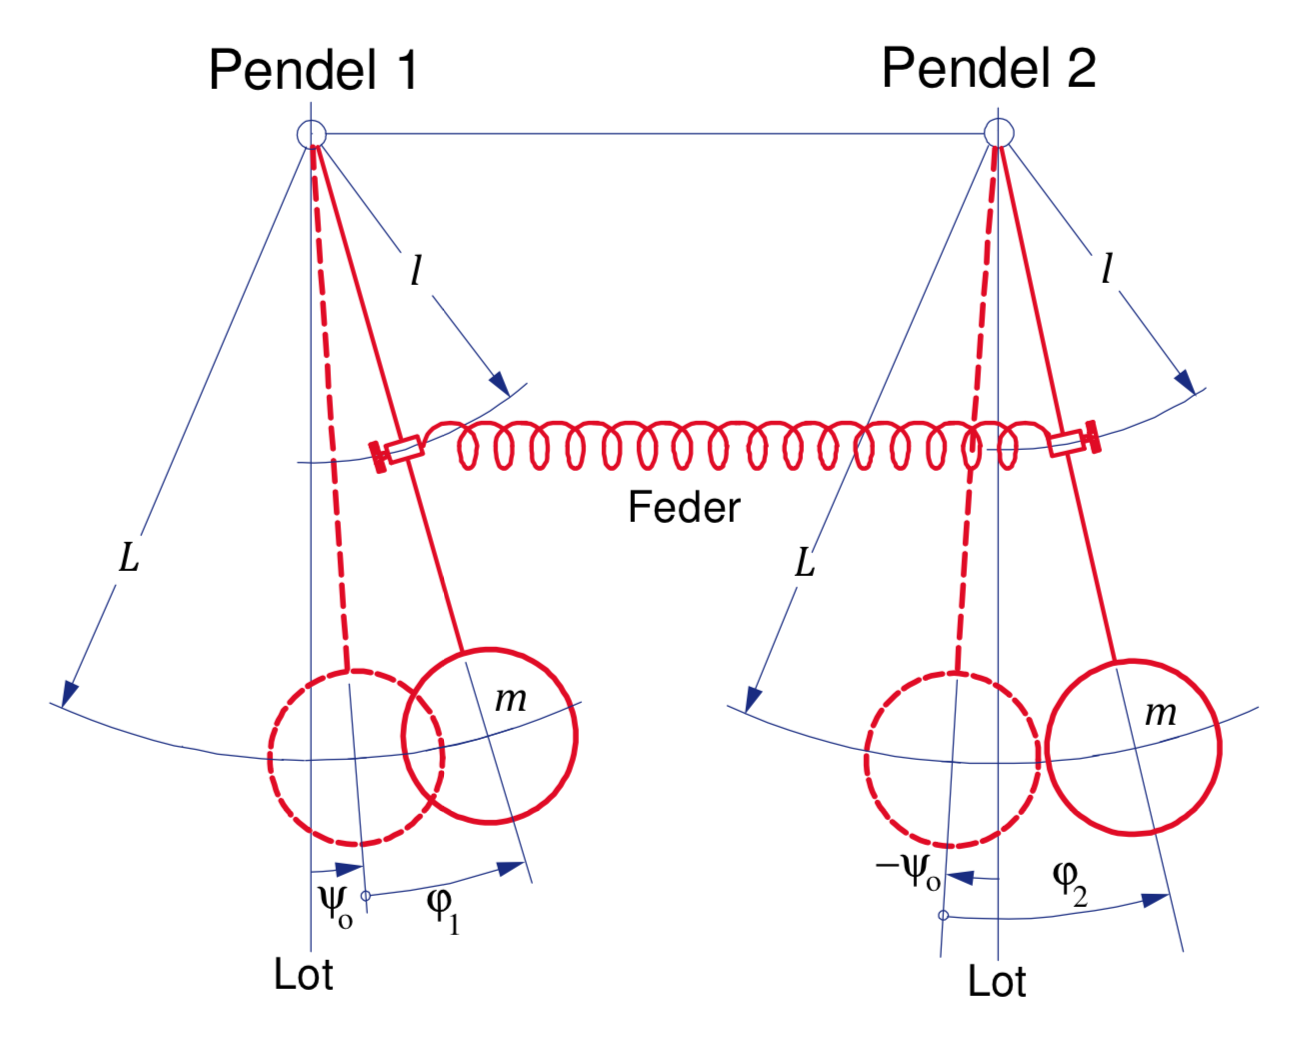
\includegraphics[width=0.9\textwidth]{ndp}}
   \renewcommand\thefigure{B1}
\caption[Gekoppeltes Pendel]{Gekoppeltes Pendel \cite{Anleitung}}
\label{Pic:1}}

\subsection{Durchführung}

% describe exp.
Wir haben zuerst 20 Schwingungsperioden einer :
\begin{itemize}
	\item Glei
\end{itemize}

\subsection{Auswertung}

XXXX

\section{Diskussion}

XXXX

\pagebreak

\section{Anhang: Tabellen und Diagramme}

\begin{table}[h]
\centering
\caption{XXXX} \vspace{11pt}
$\begin{array}{l}
\textrm{Unsicherheiten:}\\
\textrm{XXXX: } \pm XX \textrm{XX}\\
\end{array}$
\begin{tabular}{ccc}
\toprule
\textrm{XXXX}/\textrm{XX} & \textrm{XXXX}/\textrm{XX} & \textrm{XXXX}/\textrm{XX} \\
\midrule 
2 & 0.26 & 0.23\\
\hline
4 & 0.33 & 0.25\\
\hline 
5 & & 0.3\\
\hline 
6 & 1.25 & 0.83\\
\hline 
8 & 3.9 & 0.83\\ 
\hline
9 & 4.75 & 4.6\\ 
\hline
10 & 4.7 &\\ 
\bottomrule
\end{tabular}
\phantom{$\begin{array}{l}
\textrm{Unsicherheiten:}\\
\textrm{XXXX: } \pm XX \textrm{XX}\\
\end{array}$}
\label{Tab:X}
\end{table}

\begin{figure}[p]
\centering
\fbox{\includegraphics[width=0.8\textwidth]{NAME}}
\renewcommand\thefigure{BX}
\caption[XXXX]{XXXX}
\label{Abb:X}
\end{figure}

\begin{thebibliography}{9}
\bibitem{Uncertainties}''Correlations between variables are automatically handled, which sets this module apart from many existing error propagation codes.'' - https://pythonhosted.org/uncertainties/
\bibitem{Anleitung} Physikalisches Institut der Albert-Ludwigs-Universität Freiburg (Hrsg.) (08/2018): Versuchsanleitungen zum Physiklabor für Anfänger*innen, Teil 1, Ferienpraktikum im Sommersemester 2018.
\end{thebibliography}

\end{document}